\chapter{Analisis Masalah dan Perancangan Solusi \textit{Performance Regression Analysis} menggunakan \textit{distributed tracing}}

%Pada bab ini diuraikan analisis persoalan pengumpulan data pada \textit{spreadsheet} yang telah diuraikan pada Bab I. Hasil dari bab ini digunakan untuk merancang kakas yang akan diimplementasikan seperti yang dijelaskan pada Bab IV.
%Berdasarkan 


\section{Analisis Masalah}

Seiring dengan meningkatnya kompleksitas dari aplikasi Microservice, seperti dengan meningkatnya jumlah service dan keterhubungan antar service yang ada di dalamnya, akan meningkat juga kompleksitas untuk melakukan \textit{monitoring} terhadap kinerja pada keseluruhan aplikasi Microservice. Salah satu isu penting terkait dengan kinerja adalah regresi atau penurunan terhadap kinerja. Kebutuhan untuk dengan segera menentukan penyebab utama dari regresi pada sistem menjadi penting apabila regresi terjadi pada lingkungan produksi yang langsung melayani \textit{request} dari pelanggan, sehingga apabila tidak diatasi dengan segera akan berdampak langsung terhadap pengalaman pengguna dalam menggunakan aplikasi. 

Terdapat dua pendekatan yang dapat dilakukan untuk mengatasi permasalahan regresi kinerja \citep{regression-detection}, yaitu:
\begin{enumerate}
	\item Deteksi regresi dilakukan setelah aplikasi selesai dikembangkan dan di-\textit{deploy} pada lingkungan terdedikasi
	\item Deteksi regresi dilakukan sebelum aplikasi selesai dikembangkan dan di-\textit{deploy} dan melakukan studi terhadap perubahan yang dihasilkan pada \textit{source code}
\end{enumerate}  

Mengingat sifat dari Microservice yang terdistribusi, akan menjadi sulit bagi \textit{developer} jika pendeteksian regresi dilakukan dengan pendekatan individual pada masing-masing service yang ada terlebih ketika jumlah service yang ada sudah sangat banyak dan hubungan interdependensi antar service menjadi rumit. Oleh karena itu, untuk mengatasi regresi kinerja pada aplikasi berbasis Microservice, dibutuhkanlah pendekatan yang tidak mengharuskan \textit{developer} untuk melakukan pencarian sumber masalah pada masing-masing service secara individu. Sehingga pada kasus deteksi dan analisis regresi kinerja aplikasi berbasis Microservice, pendekatan pertama lebih cocok untuk digunakan.

Salah satu teknologi yang dapat digunakan untuk melakukan \textit{monitoring} dan analisis regresi pada sebuah sistem terdistribusi seperti Microservice adalah \textit{distributed tracing}. Dengan bantuan mekanisme \textit{span} dari \textit{trace}, metrik-metrik kinerja dalam aplikasi berbasis Microservice dapat dilacak secara menyeluruh. Dalam kasus penggunaan seperti yang telah disebutkan sebelumnya, \textit{distributed tracing} cocok untuk digunakan dalam melakukan analisis regresi kinerja atau \textit{Performance Regression Analysis} dalam sebuah aplikasi berbasis Microservice sebab \textit{developer} tidak perlu menganalisis satu per satu \textit{service} yang ada terutama setelah \textit{service} sudah di-\textit{deploy}.

%Salah satu teknologi yang dapat menyediakan \textit{developer} kakas untuk melakukan \textit{monitoring} sebuah sistem terdistribusi secara keseluruhan adalah \textit{distributed tracing}. Dengan memanfaat

Oleh karena itu, dapat dirumuskan alur kerja yang harus dilakukan oleh sistem \textit{Performance Regression Analysis} (PRA) sebagai berikut:
\begin{enumerate}
	\item Sistem harus dapat mendeteksi ketika terjadi regresi pada aplikasi berbasis Microservice
	\item Sistem harus dapat menentukan sumber atau akar permasalahan dari regresi setelah terdeteksi
\end{enumerate}

%Untuk dapat melakukan 

%Adapun, langkah-langkah berikut dapat dilakukan untuk melakukan analisis penyebab regresi kinerja pada Microservice \citep{parker2020distributed}:
%\begin{enumerate}
%	\item Tentukan \textit{baseline} atau pengukuran dasar dari beberapa kinerja service
%	\item Ten
%\end{enumerate}

Sudah terdapat beberapa pendekatan yang dapat digunakan untuk melakukan analisis regresi seperti yang ada pada subbab \ref{ch2-algo}. Melihat kebutuhan dari sistem PRA di atas, dari beberapa pendekatan yang ada pada subbab tersebut, penulis menilai ada dua pendekatan yang dapat digunakan yaitu pendekatan Analisis Kumulatif pada \ref{approach-cumulative} dan pendekatan Analisis Agregasi dan Korelasi pada \ref{approach-corr}. Analisis Kumulatif dapat digunakan untuk menentukan apakah telah terjadi regresi pada aplikasi dengan melakukan perbandingan antara CDF \textit{baseline} dengan CDF dari aplikasi yang sedang berjalan. Ketika didapatkan statistik K-S yang melebihi \textit{treshold}, sistem PRA akan melakukan analisis akar permasalahan dengan metode Analisis Agregasi dan Korelasi untuk mendapatkan penyebab dari regresi melalui analisis \textit{crtical path} pada \textit{service} yang terdeteksi memiliki koefisien korelasi tinggi. Penghitungan koefisien korelasi dapat dilakukan dengan menghitung koefisien korelasi antara hasil \textit{trace} ketika terdeteksi regresi dengan hasil \textit{trace} dari waktu beberapa jam sebelumnya yang masih terhitung normal sehingga data \textit{trace} tidak perlu disimpan seperti model CDF \textit{baseline}.


\begin{figure}[htb]
	\centering
	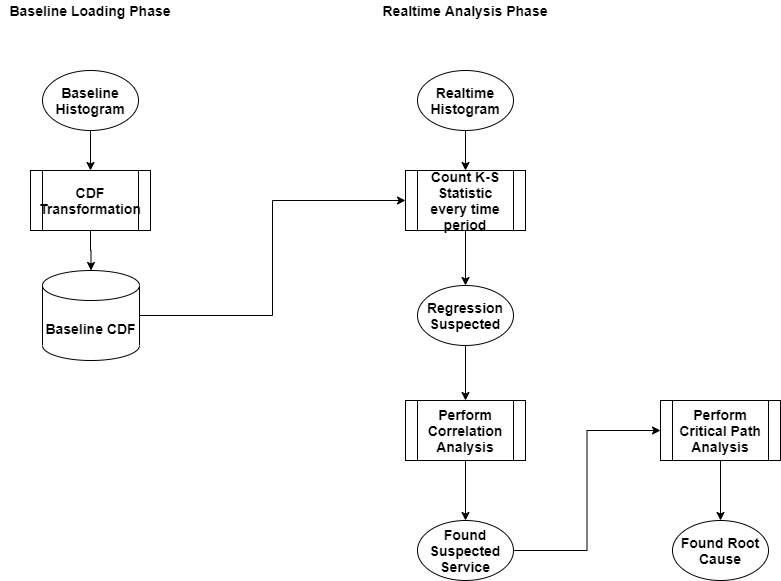
\includegraphics[width=0.6\textwidth]{resources/ch3/alur.jpg}
	\caption{Alur sistem PRA}
	\label{aur-pra}
\end{figure}




%Melihat kebutuhan untuk melakukan deteksi regresi secara terdistribusi pada Microservice, penulis menilai bahwa \textit{distributed tracing} dapat digunakan sebagai solusi untuk menyelesaikan masalah tersebut. Beberapa 


%ketika terjadi penurunan pada kinerja ataupun terdapat \textit{error} yang diakibatkan oleh suatu service tertentu.
%
%
%Regresi dalam sebuah sistem terdistribusi dapat diakibatkan oleh beberapa hal, contohnya adalah 
%\section{Analisis Alternatif Solusi} %Ngebandingin 

\section{Rancangan Solusi}

\subsection{Desain \textit{Payload}}

\subsection{Aristektur Solusi}

%\section{Rancangan Pengukuran \textit{Overhead}} % Di Bab 4

 \section{Jadwal Pelaksanaan}
 \newsavebox\mybox
 \begin{lrbox}{\mybox}
	     \begin{ganttchart}[
		     vgrid={*{6}{draw=none}, dotted},
		     x unit=.05cm,
		     y unit title=.6cm,
		     y unit chart=.6cm,
		     time slot format=isodate,
		     time slot format/start date=2016-09-01]{2021-09-01}{2022-04-30}
		     \ganttset{bar height=.6}
		     \gantttitlecalendar{year, month} \\
		     \ganttbar[bar/.append style={fill=blue}]{Studi Literatur}{2021-09-01}{2021-11-30}\\
		     \ganttbar[bar/.append style={fill=blue}]{Analisis Masalah}{2021-10-01}{2021-11-15}\\
		     \ganttbar[bar/.append style={fill=blue}]{Perancangan Solusi}{2021-11-01}{2021-12-15}\\
		     \ganttbar[bar/.append style={fill=blue}]{Implementasi}{2021-12-15}{2022-03-01}\\
		     \ganttbar[bar/.append style={fill=blue}]{Pengujian dan Analisis Hasil}{2022-02-01}{2022-04-30}
		     \end{ganttchart}
	 \end{lrbox}

 Pengerjaan tugas akhir ini direncanakan mulai pada September 2021 sampai April 2022. Pelaksanaan tugas akhir ini dibagi menjadi 5 tahap yang dapat dipetakan kepada metodologi pengerjaan sebagai berikut,
 \begin{enumerate}
	     \item Tahap 1: Studi Literatur
	     \item Tahap 2: Analisis Masalah
	     \item Tahap 3: Perancangan Solusi
	     \item Tahap 4: Implementasi
	     \item Tahap 5: Pengujian dan Analisis Hasil
	 \end{enumerate}
 Jadwal pelaksanaan tugas akhir berdasarkan metodologi pengerjaan tugas akhir dapat dilihat pada Tabel \ref{Gantt-Chart} dibawah ini.
 \begin{table}[htb]
	 \centering
	 \caption{Gantt Chart jadwal pelaksanaan tugas akhir}
	 \label{Gantt-Chart}
	 \tikz{
		   \node[inner sep=0pt,outer sep=0pt] (gantt)
		   {\begin{tabular}{c}
				     \toprule
				     \resizebox{\textwidth}{!}{\usebox\mybox} \\
				     \bottomrule
				    \end{tabular}%
			    };
		 }   
	 \end{table}

% Pada masa sebelum adopsi arsitektur Microservice dan kebanyakan dari aplikasi masih menggunakan arsitektur Monolith, proses seperti \textit{debugging} adalah hal yang sederhana sebab jika terdapat suatu \textit{error} akan mudah untuk ditelusuri dari mana asal \textit{error} tersebut sebab hanya ada satu aplikasi yang digunakan. Hal tersebut tidak berlaku jika aplikasi menggunakan model Sistem Terdistribusi, salah satu contohnya adalah Microservice. Sifat dari Microservice yang melakukan \textit{decoupling} aplikasi menjadi bagian yang lebih kecil membuat proses \textit{debugging} menjadi tidak mudah sebab untuk mencari penyebab \textit{error} aplikasi yang terdistribusi, kita harus mengetahui terlebih dahulu sumber dari \textit{error} tersebut. Kompleksitas akan bertambah dalam proses debugging jika ternyata ditemukan bahwa sautu \textit{error} pada sebuah \textit{service} bukanlah akar atau penyebab utama dari \textit{error} tersebut melainkan suatu \textit{service} lainnya. Kompleksitas akan bertambah jika metode \textit{debugging} yang digunakan mengharuskan \textit{developer} yang menangani \textit{error} tersebut harus menelusuri satu per satu \textit{service} yang terdampak sampai menemukan akar dari masalahnya. Dari masalah tersebutlah timbul suatu kebutuhan untuk mendapatkan gambaran mengenai \textit{state} sebuah Sistem Terdistribusi ataupun yang disebut juga dengan \textit{observability}.
% 
% 
% 
% Dengan bantuan dari \textit{trace} atau yang disebut \textit{distributed tracing}, \textit{developer} bisa mendapatkan suatu gambaran dari masing-masing \textit{request} yang terjadi pada sebuah \textit{resource} atau komponen yang berinteraksi dengan komponen lainnya dalam sebuah Sistem Terdistribusi seperti \textit{node}, \textit{service}, \textit{network}, ataupun \textit{mutex}. Ide dasar dari \textit{tracing} seperti yang sudah dijelaskan pada \ref{bab2-dtracing} adalah dengan mengidentifikasi sebuah titik spesifik, dapat jadi sebuah pemanggilan \textit{remote procedure call} (RPC), dalam sebuah aplikasi, \textit{library}, ataupun \textit{middleware} dalam jalur sebuah \textit{request} yang merepresentasikan kedua hal berikut:
% \begin{enumerate}
% \item \textit{Fork} pada eksekusi di level Sistem Operasi
% \item Sebuah lompatan atau akses horizontal ke luar melalui jaringan
%\end{enumerate}
%
%Data hasil \textit{trace} yang berisi kumpulan \textit{span} kemudian direpresentasikan sebagai \textit{directed acylic graph} (DAG), yang mana \textit{edge} antar graf dalam DAG yang disebut dengan \textit{reference} merepresentasikan hubungan atau kausalitas antar komponen dalam sebuah \textit{cluster} sistem terdistribusi yang terjadi pada \textit{request}. 
%
%
%
%Dengan meningkatkan performa \textit{baseline} pada sistem, para \textit{developer} berharap dapat meningkatkan kepuasan pelanggan, menurunkan biaya infrastruktur, ataupun keduanya. Untuk aplikasi yang langsung melayani pelanggan, performa seringkali berarti \textit{latency} dari \textit{request}. Proses optimisasi seperti ini biasanya adalah proses bertahap yang membutuhkan waktu.
%
%Kakas yang digunakan untuk membantu mencapai \textit{observability} penting untuk meningkatkan performa \textit{baseline} dengan pertama kali mengukur performa awal yang menjadi \textit{baseline} pengukuran dan digunakan untuk mengarahkan para \textit{developer} agar dapat mencari bagian mana dari aplikasi yang dapat ditingkatkan performanya. Dengan aplikasi yang menggunakan arsitektur Monolith, para \textit{developer} dapat dengan mudah melakukan \textit{profiling} proses mana saja yang dapat ditingkatkan penggunaan \textit{resource}-nya seperti CPU ataupun Memory. Namun dengan penggunaan arsitektur Microservice yang berbasis sistem terdistribusi, terkadang sulit untuk mengetahui \textit{service} manakah yang tepatnya perlu ditingkatkan penggunaan \textit{resource}-nya, sehingga penggunaan \textit{distributed tracing} akan sangat membantu untuk meningkatkan performa \textit{baseline} dari sebuah sistem terdistribusi.
%
%Berbeda dengan tujuan untuk meningkatkan performa \textit{baseline}, tujuan lainnya yaitu untuk mengembalikan performa \textit{baseline} bukanlah suatu hal yang dapat begitu saja direncanakan. Regresi dalam performa dapat muncul tiba-tiba seperti terjadinya \textit{outtage} atau pemberhentian tiba-tiba dari sebuah \textit{cluster} sistem terdistribusi. Melihat sifat dari sistem terdistribusi, mencari penyebab utama dari sebuah \textit{outtage} bukanlah sebuah hal yang mudah terlebih jika ada ratusan bahkan ribuan \textit{node} yang terdapat pada \textit{cluster} dan masing-masing \textit{node} saling terhubung dengan yang lainnya. Jika hal semacam tersebut terjadi dalam lingkungan aplikasi \textit{production} maka dampaknya akan terasa langsung oleh pelanggan dan dalam jangka panjang dapat menimbulkan kerugian material. Oleh karena itu, penting untuk segera mengetahui sumber atau akar dari suatu kejadian yang menyebabkan regresi pada performa sistem.
%
%Dari solusi \textit{distributed tracing} bersifat \textit{open source} yang tersedia saat ini, Zipkin dan Jaeger adalah dua solusi \textit{tracing} yang sudah menyediakan komponen instrumentasi, \textit{deployment}, dan \textit{value delivery} dalam bentuk \textit{application programming interface} (API) dan \textit{user interface} secara \textit{default}. Berikut adalah tabel perbandingan dari fitur \textit{user interface} web Zipkin dan Jaeger.
%
%
%\begin{small}
%	\begin{longtable}{ | p{3.75cm} | p{5.5cm} | p{5.5cm} | }
%		\caption{Deskripsi Perbandingan fitur Zipkin dan Jaeger}
%		\label{jzipkin-comparison}                                                                                                                \\ \hline
%		 & \centering\bfseries{Jaeger \citep{jaeger}} & \centering\bfseries{Zipkin \citep{zipkin}} \tabularnewline \hline
%		\endfirsthead
%		\bfseries{Deskripsi Singkat} & Dirilis sebagai kakas \textit{open-source} oleh Uber Technologies. Jaeger digunakan untuk melakukan \textit{monitoring} dan \textit{troubleshoot} dari sistem terdistribusi yang berbasis Microservice & Membantu mengumpulkan data bersifat temporal yang dibutuhkan untuk melakukan \textit{troubleshoot} permasalahn \textit{latency} pada aplikasi Microservice. Zipkin mengatur pengoleksian dan juga pencarian data. Desain dari Zipkin dibuat berdasarkan \textit{paper} dari Daper \citep{dapper-paper}\\ \hline
%		\bfseries{Kelebihan} &  \textit{Open-source}; 
%		Siap digunakan dengan Docker; Antarmuka dari \textit{collector} cocok digunakan dengan protokol milik Zipkin; Tingkat \textit{sampling} yang bersifat dinamis; Memiliki antarmuka berbasis Web &  \textit{Open-source}; 
%		Siap digunakan dengan Docker; Dapat menggunakan teknologi transport bagi \textit{span} yang berbeda-beda (HTTP, Kafka, Scribe, AMQP); Memiliki antar muka berbasis Web  \\ \hline
%		\bfseries{Kekurangan} & Hanya mendukung dua teknologi transport untuk \textit{span} (Thrift dan HTTP) & Tingkat \textit{sampling} yang bersifat \textit{fixed} \\ \hline
%		\bfseries{Jenis Analisis tersedia} & Visualisasi graf dependensi; Perbandingan hasil \textit{trace} & Visualisasi graf dependensi \\ \hline
%	\end{longtable}
%\end{small}
%
%Dari pemaparan mengenai kedua tujuan dari \textit{observability} di atas dan berdasarkan studi terhadap solusi \textit{open-source} yang sudah ada, penulis menyimpulkan bahwa ada dua hal yang dapat dibuat dengan menggunakan \textit{distributed tracing} untuk mencapai kedua tujuan utama dari \textit{observability}:
%\begin{enumerate}
%	\item Membuat Service Map untuk mencapai tujuan pertama yaitu meningkatkan performa baseline
%	\item Membuat perangkat untuk melakukan Root Cause Analysis (RCA) untuk mencapai tujuan kedua yaitu mengembalikan performa baseline ketika terjadi regresi pada sistem
%\end{enumerate}
%
%Service Map merupakan visualisasi dari sebuah sistem Microservice yang melakukan dekomposisi pada semua komponen \textit{service} dan menggambarkan dependensi yang terlihat antar \textit{service} tersebut secara \textit{real-time}, sehingga \textit{developer} dapat mengidentifikasi \textit{bottleneck} yang ada dan memahami bagaimana data mengalir dalam aristektur \citep{datadog-svcmap}. Untuk dapat membantu meningkatkan performa \textit{baseline}, sebuah Service Map harus dapat menyediakan informasi mengenai hubungan interdependensi antara \textit{service}, jumlah \textit{request} yang diterima oleh service per satuan waktu, dan ukuran performa pada \textit{service} tersebut dalam merespon \textit{service} lainnya. Ukuran performa yang dapat dijadikan \textit{baseline} antara lain adalah \textit{latency}, \textit{failure rate}, \textit{traffic rate}, dan saturasi, namun biasanya \textit{developer} hanya berfokus pada pengukuran \textit{latency} dan \textit{failure rate} \citep{parker2020distributed}.
%
%Selain digunakan untuk mendapatkan gambaran mengenai komponen yang ada pada suatu \textit{cluster} sistem terdistribusi, salah satu pendekatan yang dapat digunakan oleh Service Map untuk meningkatkan performa \textit{baseline}  disebut \textit{Correlation Analysis} \citep{parker2020distributed}. Untuk melakukan \textit{Correlation Analysis}, dibutuhkan tidak hanya satu tetapi dua sampel dari \textit{trace}. Satu sampel harus dapat merepresentasikan kelas \textit{trace} yang hendak dieliminasi atau setidaknya dikurangi jumlahnya, contohnya \textit{request} yang gagal atau lambat. Sampel jenis kedua harus dapat merepresentasikan komplemen dari sampel yang pertama, biasanya sekelompok \textit{request} yang cepat atau sukses. Selain dari dua kelompok sampel tadi, dibutuhkan juga sekelompok fitur yang dapat dicari korelasinya. Fitur-fitur yang dicari dalam sebuah sistem terdistribusi antara lain adalah \textit{service}, operasi, \textit{error}, dan \textit{tag} yang berasosiasi dengan \textit{span} yang membuat \textit{trace} tersebut. 
%
%Setelah dimiliki dua kelompok sampel (misal sampel A dan B) dan juga sekelompok fitur, analisis dilakukan dengan melihat setiap fitur dan mengajukan pertanyaan "Apa kemungkinan fitur tersebut ada pada sampel A tetapi tidak ada di sampel B?". Pertanyaan tersebut akan menghasilkan "koefisien korelasi" bagi setiap fitur. Koefisien yang bernilai 1.0 berarti sebuah fitur ada pada setiap \textit{trace} pada sampel A dan tidak pernah ada pada sebuah \textit{trace} di sampel B, sementara koefisien -1.0 berarti sebuah fitur yang ada pada setiap \textit{trace} di sampel B dan tidak pernah ada pada \textit{trace} di sampel A. Sebuah koefisien 0.0 berarti fitur tersebut secara seimbang dapat ada pada kedua sampel. Semakin dekat hasil ke 1.0 atau -1.0 sebuah koefisien korelasi, semakin mungkin sebuah fitur dapat menjelaskan perbedaan antara kedua sampel. 
%
%Di sisi lain, kakas untuk melakukan Root Cause Analysis dapat digunakan untuk memberikan petunjuk kepada \textit{developer} mengenai komponen mana dari Microservice yang mengalami regresi sehingga \textit{developer} dapat mengatasi permasalahan tersebut dengan segera. Salah satu pendekatan yang bisa dilakukan untuk mengembalikan performa adalah dengan pendekatan \textit{Aggregate and Correlation Root Cause Analysis} \citep{parker2020distributed}. Tidak jauh berbeda dengan pendekatan yang telah terlebih dahulu disebutkan pada Service Map, pendekatan ini menggunakan agregasi dari beberapa \textit{trace} untuk mendapatkan koefisien korelasi mengenai keadaan performa sebuah \textit{service}. 
%
%Adapun dari pemaparan di atas mengenai fitur analisis \textit{distributed tracing}, penulis menyimpulkan kebutuhan fungsional apa saja yang diperlukan pada pembuatan kakas visualisasi \textit{distributed tracing}:
%
%\begin{small}
%	\begin{longtable}{ | p{2cm} | p{10cm} | }
%		\caption{Kebutuhan Fungsional kakas visualisasi}
%		\label{fr-vis}                                                                                                                     \\ \hline
%		\centering\bfseries{ID} & \centering\bfseries{Deskripsi} \tabularnewline \hline
%		\endfirsthead
%		\hline
%		\centering\bfseries{ID} & \centering\bfseries{Deskripsi} \tabularnewline \hline
%		\endhead
%		FR-01 & Kakas dapt menampilkan hubungan interdependensi antara \textit{service} \\ \hline
%		FR-02 & Kakas dapat menampilkan pengukuran performa \textit{latency} pada setiap \textit{service} \\ \hline
%		FR-03 & Kakas dapat melakukan \textit{Correlation Analysis} untuk menentukan komponen mana dari Microservice yang dapat ditingkatkan performanya \\ \hline
%		FR-04 & Kakas dapat melakukan Root Cause Analysis (RCA) ketika terjadi sebuah regresi pada sistem dengan menggunakan pendekatan \textit{Aggregate and Correlation Root Cause Analysis} \\ \hline
%	\end{longtable}
%\end{small}






%Untuk mencapai kedua tujuan dari \textit{observability} tersebut, \textit{distributed tracing} dapat digunakan untuk menyediakan hal-hal berikut:
%\begin{enumerate}
%	\item 
%\end{enumerate}



%Seiring dengan meningkatnya penggunaan arsitektur, mengingkat pula kebutuhan bagi para \textit{developer} untuk dapat dengan segera mengetahui sumber dari permasalahan jika terjadi \textit{error} pada sistem.
%
%Dari pemaparan mengenai masih kurangnya kakas visualisasi \textit{tracing} yang bersifat \textit{open source}
%. Berdasarkan studi literatur mengenai \textit{observability} untuk Sistem Terdistribusi pada \ref{bab2-observability}, terdapat 

%Isu visualisasi 
%Overhead


